\documentclass[11pt,a4paper]{article}

% -----------------------------------------------------------------------------
% Typography and page design
% -----------------------------------------------------------------------------
\usepackage[T1]{fontenc}
\usepackage[utf8]{inputenc}
\usepackage{newtxtext}
\usepackage{amsthm}
\usepackage{newtxmath}
\usepackage[scaled=0.94]{inconsolata}
\usepackage{microtype}
\usepackage[a4paper,margin=25mm,headheight=15pt]{geometry}
\usepackage{setspace}
\setstretch{1.06}
\usepackage{parskip}
\setlength{\parindent}{0pt}
\usepackage{fancyhdr}
\usepackage{lastpage}
\usepackage{titlesec}
\usepackage{xcolor}
\definecolor{Forest}{HTML}{173F35}
\definecolor{Moss}{HTML}{52796F}
\definecolor{Earth}{HTML}{8A5A44}
\definecolor{Rust}{HTML}{9B3A2E}
\definecolor{Mist}{HTML}{EEF3F1}
\definecolor{Sand}{HTML}{F5F0E7}
\definecolor{Ink}{HTML}{172026}
\definecolor{Slate}{HTML}{5D6870}
\color{Ink}

\titleformat{\section}
  {\Large\bfseries\color{Forest}}{\thesection}{0.65em}{}
\titleformat{\subsection}
  {\large\bfseries\color{Earth}}{\thesubsection}{0.6em}{}
\titleformat{\subsubsection}
  {\normalsize\bfseries\color{Ink}}{\thesubsubsection}{0.55em}{}
\titlespacing*{\section}{0pt}{2.2ex plus .5ex}{0.9ex}
\titlespacing*{\subsection}{0pt}{1.8ex plus .4ex}{0.6ex}

\pagestyle{fancy}
\fancyhf{}
\fancyhead[L]{\small\textsc{Nash's Cage / RVCIM}}
\fancyhead[R]{\small\textsc{Preprint Draft v0.2}}
\fancyfoot[L]{\small SpiralReality with Ry\={o} $\therefore$ SpiralArchitect}
\fancyfoot[R]{\small \thepage\ / \pageref{LastPage}}
\renewcommand{\headrulewidth}{0.4pt}
\renewcommand{\footrulewidth}{0pt}

% -----------------------------------------------------------------------------
% Mathematics, tables, figures, and references
% -----------------------------------------------------------------------------
\usepackage{mathtools,bm}
\numberwithin{equation}{section}
\usepackage{booktabs,tabularx,longtable,array,multirow}
\newcolumntype{Y}{>{\raggedright\arraybackslash}X}
\newcolumntype{C}{>{\centering\arraybackslash}X}
\newcolumntype{L}[1]{>{\raggedright\arraybackslash}p{#1}}
\usepackage{enumitem}
\setlist[itemize]{leftmargin=1.35em,itemsep=0.25em,topsep=0.35em}
\setlist[enumerate]{leftmargin=1.55em,itemsep=0.25em,topsep=0.35em}
\usepackage{graphicx}
\usepackage{caption}
\captionsetup{font=small,labelfont=bf}
\usepackage{float}
\usepackage{tikz}
\usetikzlibrary{arrows.meta,positioning,fit,calc,shapes.geometric,backgrounds}
\usepackage[most]{tcolorbox}
\tcbset{boxrule=0.6pt,arc=2mm,left=3mm,right=3mm,top=2mm,bottom=2mm}
\newtcolorbox{corebox}{colback=Mist,colframe=Forest,title=Core claim,fonttitle=\bfseries}
\newtcolorbox{boundarybox}{colback=Sand,colframe=Earth,title=Claim boundary,fonttitle=\bfseries}
\newtcolorbox{warningbox}{colback=Rust!5,colframe=Rust,title=Failure mode,fonttitle=\bfseries}
\newtcolorbox{provenancebox}{colback=Mist,colframe=Moss,title=Revision provenance,fonttitle=\bfseries}

\usepackage{listings}
\lstdefinestyle{paperpseudo}{
  basicstyle=\ttfamily\small,
  frame=single,
  rulecolor=\color{Moss},
  backgroundcolor=\color{Mist!55},
  breaklines=true,
  columns=fullflexible,
  xleftmargin=0.5em,
  framexleftmargin=0.5em,
  keywordstyle=\bfseries\color{Forest},
  commentstyle=\itshape\color{Slate},
  showstringspaces=false
}

\usepackage{url}
\usepackage[colorlinks=true,linkcolor=Forest,citecolor=Earth,urlcolor=Moss]{hyperref}
\hypersetup{
  pdftitle={Nash's Cage: Robust Viability-Constrained Payoff-Inversion Governance under Unknown Irreversible Boundaries},
  pdfauthor={SpiralReality with Ryo - SpiralArchitect},
  pdfsubject={A formal research proposal with an executable F0 reference model for robust viability-constrained climate governance},
  pdfkeywords={Nash equilibrium, dynamic games, climate governance, viability theory, robust control, institutional capture, tipping points, deep uncertainty}
}
\usepackage[backend=bibtex,style=authoryear,natbib=true,maxcitenames=2,maxbibnames=99,doi=true,url=true,isbn=false]{biblatex}
\addbibresource{references.bib}
\renewcommand*{\bibfont}{\small}
\usepackage[capitalise,noabbrev]{cleveref}

% -----------------------------------------------------------------------------
% Theorem-like environments
% -----------------------------------------------------------------------------
\theoremstyle{definition}
\newtheorem{definition}{Definition}[section]
\newtheorem{designprinciple}[definition]{Design Principle}
\newtheorem{hypothesis}[definition]{Hypothesis}
\theoremstyle{plain}
\newtheorem{proposition}[definition]{Proposition}
\theoremstyle{remark}
\newtheorem{remark}[definition]{Remark}

% -----------------------------------------------------------------------------
% Commands
% -----------------------------------------------------------------------------
\newcommand{\R}{\mathbb{R}}
\newcommand{\E}{\mathbb{E}}
\newcommand{\Pp}{\mathbb{P}}
\newcommand{\ind}{\mathbb{I}}
\newcommand{\argmax}{\operatorname*{arg\,max}}
\newcommand{\argmin}{\operatorname*{arg\,min}}
\newcommand{\Proj}{\operatorname{Proj}}
\newcommand{\Viab}{\operatorname{Viab}}
\newcommand{\diag}{\operatorname{diag}}
\newcommand{\cage}{\mathsf{Cage}}
\newcommand{\RVCIM}{\textsc{RVCIM}}
\newcommand{\safe}{\mathcal{X}_{\mathrm{safe}}}
\newcommand{\irrev}{\mathcal{X}_{\mathrm{irr}}}
\newcommand{\policy}{\boldsymbol{\pi}}
\newcommand{\state}{\bm{x}}
\newcommand{\kpi}{\bm{k}}
\newcommand{\action}{\bm{a}}
\newcommand{\capture}{\bm{c}}
\newcommand{\inst}{\bm{\iota}}
\newcommand{\narr}{\bm{n}}

\begin{document}

% -----------------------------------------------------------------------------
% Title page
% -----------------------------------------------------------------------------
\hypersetup{pageanchor=false}
\begin{titlepage}
\thispagestyle{empty}
\centering
\vspace*{1.6cm}
{\small\bfseries\color{Moss}\MakeUppercase{Conceptual Paper / Preprint Draft}}\\[1.1cm]
{\fontsize{31}{36}\selectfont\bfseries\color{Forest} Nash's Cage}\\[0.55cm]
{\fontsize{17}{22}\selectfont\color{Earth}
Robust Viability-Constrained Payoff-Inversion Governance\\
under Unknown Irreversible Boundaries}\\[1.6cm]

{\Large\textsc{SpiralReality}}\\[0.35cm]
{\large Conceptual architecture with Ry\={o} $\therefore$ SpiralArchitect}\\[1.5cm]

\begin{tcolorbox}[width=0.84\textwidth,colback=Mist,colframe=Forest,boxrule=0.8pt]
\centering\large\bfseries
Civilization is optimizing inside an unknown viability boundary.
\end{tcolorbox}

\vfill
{\large Regenerated revision v0.2}\\[0.2cm]
{\large 7 August 2026}\\[1cm]
{\small This manuscript is a formal research proposal, not a claim of empirical validation or a finished institutional design.}
\end{titlepage}
\hypersetup{pageanchor=true}
\setcounter{page}{1}

% -----------------------------------------------------------------------------
% Abstract and navigation
% -----------------------------------------------------------------------------
\begin{abstract}
Climate governance is commonly framed as a cooperation problem in which individually rational actors underprovide a global public good. That framing is useful but incomplete. It does not, by itself, represent endogenous institutional delay, strategic metric manipulation, symbolic compliance, unequal externalization capacity, uncertain recovery boundaries, or the possibility that governance capacity deteriorates while physical risk accumulates. This paper introduces \emph{Nash's Cage}: a partially observable, capture-prone stochastic dynamic game in which self-interested agents optimize short-horizon payoffs while externalizing physical and social constraints, thereby shrinking a robust viability region faster than institutions can observe, coordinate, and respond.

We formalize a companion architecture, the \emph{Robust Viability-Constrained Cage-Inversion Model} (\RVCIM). The model combines heterogeneous agent utilities, a manipulable KPI observation layer, endogenous institutional actuators, narrative dynamics, adversarial capture, model ambiguity, a robust viability kernel, and a braking-time measure termed \emph{controllability reserve}. Four conditional propositions isolate the architecture's central claims: monitoring without institutional coupling is performative; capture can dominate nominal triggers; non-positive braking reserve removes a robust certificate of timely response and, under a separately declared precautionary rule, triggers escalation; and cooperation becomes locally rational only when the payoff differential is inverted for a decisive coalition. Viability and justice are treated as hard constraints rather than fungible terms in a welfare sum.

The paper then specifies accountable automatic triggers, anti-capture separation of powers, multimodal ecological sensing, and dynamic policy pathways. Soundscape metrics are included only as one candidate sensor within a multimodal ensemble requiring site-specific validation. A red-team catalogue describes realistic adaptations by regulated actors and corresponding defenses. Finally, we state falsifiable hypotheses, a simulation program, and an executable F0 reference contract. The contribution is not a proof that a particular climate treaty must fail, nor a claim that one universal controller can govern Earth. It is a formal specification for asking whether a governance system preserves the capacity to brake before unknown irreversible boundaries become operationally unreachable.
\end{abstract}

\noindent\textbf{Keywords:} dynamic games; climate governance; viability theory; robust control; institutional capture; tipping points; deep uncertainty; control barrier functions; soundscape ecology; just transition.

\vspace{0.8em}
\begin{boundarybox}
The term \emph{Nash's Cage} does not imply that every Nash equilibrium is socially harmful, that climate politics reduces to a two-player Prisoner's Dilemma, or that automation can replace democratic judgment. It names a narrower model class: stable strategic configurations in which local best responses reproduce collective physical degradation and degrade the future capacity to change course.
\end{boundarybox}

\begin{provenancebox}
The repository preserves the exact uploaded v0.1 source. This v0.2 is a regenerated revision dated 7 August 2026, based on that source and extended with the executable-companion contract described below. It is not represented as byte-identical to an earlier, unavailable v0.2 build. File identities and the regeneration boundary are recorded in the repository's release manifest.
\end{provenancebox}

{\small\tableofcontents}
\newpage

% -----------------------------------------------------------------------------
\section{Introduction}
% -----------------------------------------------------------------------------

A Nash equilibrium is a profile from which no player benefits by unilateral deviation, given the strategies of the others \citep{nash1950}. Stability in this sense is not equivalent to collective optimality. Common-pool resource problems, public-goods games, repeated dilemmas, and climate cooperation studies show that individually defensible choices can maintain collectively inferior outcomes \citep{hardin1968,axelrod1984,ostrom1990,milinski2008,nordhaus2015}. Yet the climate problem is more difficult than the canonical matrix game: actors are heterogeneous, actions are continuous and path dependent, observations are delayed, institutional rules change endogenously, and some actors can spend resources to reshape the rules by which they are evaluated.

The empirical context motivates, but does not prove, the model. The Paris Agreement's Article 15 mechanism is expressly expert-based, facilitative, non-adversarial, and non-punitive \citep{unfccc2015,unfcccpaicc}. UNEP's 2025 assessment estimated end-of-century warming of roughly 2.3--2.5\,\textdegree C under full implementation of current nationally determined contributions and 2.8\,\textdegree C under current policies \citep{unep2025}. The 2025 Production Gap Report found that planned 2030 fossil-fuel production remained more than twice the level associated with a 1.5\,\textdegree C pathway \citep{productiongap2025}. The WMO reported a global mean atmospheric carbon dioxide concentration of 423.9 ppm in 2024 \citep{wmo2025}. These observations are consistent with a gap between symbolic commitment and physical trajectory, but they do not by themselves identify a single causal mechanism. \RVCIM is proposed as a testable mechanism class.

\begin{corebox}
\textbf{Diagnostic thesis.} The central governance failure is not merely insufficient observation. It is weak, delayed, and manipulable coupling from physical observation to institutional response, from institutional response to agent payoffs, and from payoffs to actions that preserve future controllability.
\end{corebox}

The paper makes six contributions.

\begin{enumerate}
  \item It defines Nash's Cage as a partially observable, institutionally endogenous dynamic game rather than a static metaphor.
  \item It distinguishes physical safety, robust viability, and operational braking reserve, allowing a state to appear safe while already lacking a certified path to stop.
  \item It defines \emph{payoff coupling strength}, linking KPI changes to the utility difference between cooperation and defection.
  \item It models regulatory capture as an adversarial action vector that attacks sensors, models, actuators, delay, narratives, finance, and justice.
  \item It specifies \RVCIM, in which viability and justice are hard constraints, automatic triggers are accountable rather than discretionary, and policy pathways remain adaptive under deep uncertainty.
  \item It converts the architecture into a red-team and empirical research program with measurable failure criteria.
\end{enumerate}

% -----------------------------------------------------------------------------
\section{Foundations and Scope}
% -----------------------------------------------------------------------------

\subsection{From bad equilibrium to a dynamic cage}

The Prisoner's Dilemma is a useful local motif: if temptation exceeds mutual cooperation, mutual defection, and unilateral cooperation in the familiar ordering, defection is individually dominant while mutual cooperation is Pareto superior. Climate interactions, however, can also resemble assurance games, chicken, repeated public-goods games, bargaining games, common-pool resource games, and coalition games. Accordingly, Nash's Cage does not assert one universal payoff matrix. It asserts a dynamic property: for a decisive set of actors, the locally preferred actions reproduce degradation and resist unilateral exit.

Repeated interaction can sustain cooperation when future consequences, reputation, reciprocity, and credible punishment matter \citep{axelrod1984,ostrom1990}. Climate governance often weakens this ``shadow of the future'' through election cycles, quarterly reporting, capital turnover, jurisdictional leakage, and non-binding commitments. Climate clubs and coordinated trade measures have therefore been proposed as methods for changing free-riding incentives \citep{nordhaus2015}. \RVCIM generalizes the same intuition: the object of design is not moral exhortation but the intertemporal payoff field.

\subsection{Partial observability and endogenous institutions}

Dynamic noncooperative games explicitly represent evolving states and strategic feedback \citep{basar1999}. Partially observable decision processes distinguish the true state from the information available to the decision-maker \citep{kaelbling1998}. In planetary governance, this distinction is essential: no actor observes the complete Earth-system state, the full distribution of future thresholds, or the true degree of institutional fragility. Moreover, the observation process is not neutral. Reporting boundaries, measurement choices, lobbying, accounting rules, and narrative framing can be strategic actions.

Institutions are therefore modeled as endogenous state variables and actuators, not fixed constraints. Regulatory capture research emphasizes that regulated interests can influence agencies, information, standards, and enforcement \citep{carpentermoss2014}. Greenwashing research similarly treats symbolic environmental communication as an organizational response shaped by incentives and monitoring conditions \citep{delmasburbano2011}. In the present model, symbolic action and capture are explicit elements of the action space.

\subsection{Viability, safety, and deep uncertainty}

Viability theory studies whether a controlled dynamical system can remain within a constraint set over time \citep{aubin2011}. Control barrier functions encode safety conditions that can be enforced while pursuing performance objectives \citep{ames2017,ames2019}. Robust and adaptive decision frameworks address uncertainty in models, distributions, and future conditions; dynamic adaptive policy pathways emphasize sequencing, signposts, and switching rules rather than commitment to a single forecast \citep{haasnoot2013,kwakkel2016}.

The analogy to social governance must be used carefully. Institutions are not deterministic motors, citizens are not control inputs, and political legitimacy cannot be reduced to a quadratic program. The transfer is structural: safety should constrain optimization; uncertain boundaries require robustness; delay belongs inside the model; and a system should preserve the option to change course.

\subsection{Earth-system boundaries and irreversible risk}

Earth-system and planetary-boundary research identifies interacting biophysical processes that delimit a safe operating space \citep{rockstrom2023,richardson2023}. Climate tipping elements may exhibit threshold behavior, self-amplifying change, and hysteresis \citep{scheffer2009,armstrong2022}. The IPCC assesses increasingly severe, interconnected, and in some cases irreversible risks with additional warming \citep{ipcc2022,ipcc2023}. These literatures do not provide a single exact global cliff. They instead motivate the central uncertainty of this paper: the shape and distance of the true recovery boundary are only partially known.

% -----------------------------------------------------------------------------
\section{Model Primitives}
% -----------------------------------------------------------------------------

\subsection{State, agents, and action space}

Let time be discrete, $t=0,1,\ldots$, and let $\mathcal N=\{1,\ldots,N\}$ denote heterogeneous actors. An actor may represent a state, firm, financial institution, regulator, local government, sectoral coalition, or organized public. The full state is
\begin{equation}
  \state_t = (\bm{s}_t,\bm{z}_t,\inst_t,\narr_t),
  \label{eq:fullstate}
\end{equation}
where $\bm{s}_t$ is the physical state, $\bm{z}_t$ contains actor-specific stocks and dependencies, $\inst_t$ is the institutional state, and $\narr_t$ is the cognitive and legitimacy state.

\begin{table}[H]
\centering
\caption{Layered state representation. The variables are illustrative rather than exhaustive.}
\label{tab:layers}
\begin{tabularx}{\textwidth}{@{}L{0.18\textwidth}L{0.26\textwidth}Y@{}}
\toprule
\textbf{Layer} & \textbf{Representative variables} & \textbf{Interpretation} \\
\midrule
Physical & $C_t,B_t,X_t,L_t,W_t$ & Atmospheric forcing; biosphere integrity; tail-event intensity; infrastructure stress; water, food, and coupled life-support states. \\
Agent & $E_{i,t},F_{i,t},D_{i,t},G_{i,t}$ & Emissions; fossil dependence or production; direct decarbonization; symbolic compliance. \\
Institution & $P_t,Q_t,M_t,\tau_t,J_t$ & Penalty strength; transition support; monitoring fidelity; policy delay; justice and compensation capacity. \\
Cognition & $\Phi_t,A_t^{\mathrm{ware}},T_t^{\mathrm{rust}}$ & Dominant narrative frame; public awareness; trust and legitimacy. \\
Irreversibility & $\mathcal V_t,CR_t,\rho_t$ & Viability region; controllability reserve; robust recovery probability. \\
\bottomrule
\end{tabularx}
\end{table}

Actor $i$ chooses
\begin{equation}
  \action_{i,t}=(e_{i,t},f_{i,t},d_{i,t},g_{i,t},\ell_{i,t},r_{i,t},h_{i,t}),
  \label{eq:action}
\end{equation}
where the components denote emissions, fossil production or dependence, direct decarbonization, symbolic action, capture or delay effort, ecological restoration, and adaptation. Including $g_{i,t}$ and $\ell_{i,t}$ is essential: a model that treats performative compliance and rule-shaping as exogenous noise omits strategies that may be cheaper than physical transformation.

The physical dynamics are
\begin{equation}
  \bm{s}_{t+1}=F_{\theta}(\bm{s}_t,\action_t,\bm{\xi}_t),
  \qquad \theta\in\Theta_t,
  \label{eq:physicaldynamics}
\end{equation}
with aggregate action $\action_t=(\action_{1,t},\ldots,\action_{N,t})$, disturbance $\bm{\xi}_t$, and model index $\theta$. Illustrative components are
\begin{align}
C_{t+1} &= C_t + \sum_i e_{i,t} - \operatorname{Sink}_{\theta}(B_t,C_t,\text{heat},\text{drought},\text{fire}), \\
B_{t+1} &= B_t - \alpha C_t - \beta U_t^{\mathrm{land}}-\gamma U_t^{\mathrm{pollution}}
           -\delta U_t^{\mathrm{noise/light}} + \sum_i r_{i,t}.
\end{align}
The sink is endogenous: degradation can reduce future absorptive capacity. Tail risk is represented as
\begin{equation}
  q_{j,t}^{\mathrm{tail}}=\Pp_{\theta}\!\left(X_{j,t}>\Theta_j^{\mathrm{design}}\mid \bm{s}_t\right),
  \label{eq:tailrisk}
\end{equation}
not merely by a change in the mean. Cascades may be modeled through an interdependency graph among power, water, food, health, logistics, communications, finance, and governance.

\subsection{Utility, horizons, and externalization}

Let $\Pi_i^{\mathrm{feas}}$ denote actor $i$'s feasible policies. A generic discounted objective is
\begin{align}
U_i(\policy_i,\policy_{-i};\theta)
=\E_{\theta}\sum_{k=0}^{H_i}\beta_i^k\Big[&
G_i^{\mathrm{econ}}(e_i,f_i)
+B_i^{\mathrm{free}}(\action_{-i})
+B_i^{\mathrm{sym}}(g_i,\narr)
+Q_i(d_i,r_i;\inst,\kpi) \nonumber\\
&-C_i^{\mathrm{trans}}(d_i,r_i,h_i)
-P_i(e_i,f_i;\inst,\kpi)
-D_i(\bm{s}) \nonumber\\
&-C_i^{\mathrm{audit}}(g_i,\ell_i;M)
-C_i^{\mathrm{legal}}(\action_i;\inst)
-C_i^{\mathrm{cap}}(\ell_i)
\Big].
\label{eq:utility}
\end{align}
Short political and financial horizons are represented by small $H_i$ or low $\beta_i$. Climate damage borne by the actor is
\begin{equation}
D_i(\bm{s}_t)=E_i^{\mathrm{exposure}}V_i^{\mathrm{vulnerability}}
\eta_i^{\mathrm{internalization}}D(\bm{s}_t),
\qquad
\chi_i^{\mathrm{externalization}}=1-\eta_i^{\mathrm{internalization}}.
\label{eq:externalization}
\end{equation}
Powerful actors may lower $\eta_i^{\mathrm{internalization}}$ through insurance, relocation, price pass-through, legal privilege, supply-chain displacement, or temporal deferral. Benefits are internalized; losses are displaced across jurisdiction, class, species, or generation.

\subsection{Observation, KPI construction, and manipulation}

The true state is not directly observed. Raw observations satisfy
\begin{equation}
  \bm{y}_t=O_{\theta}(\state_t,\action_t)+\bm{\varepsilon}_t+\bm{\mu}_t,
  \label{eq:observation}
\end{equation}
where $\bm{\varepsilon}_t$ is measurement and model error and $\bm{\mu}_t$ is strategic manipulation. The institutional KPI vector is produced by a fusion operator
\begin{equation}
  \kpi_t=\mathcal H(\bm{y}_{0:t};\mathcal M_t),
  \label{eq:kpi}
\end{equation}
where $\mathcal M_t$ contains models, baselines, accounting rules, and metadata. A stylized integrity score is
\begin{equation}
\mathsf{DI}_t=
\frac{M_t^{\mathrm{fidelity}}M_t^{\mathrm{independence}}M_t^{\mathrm{comparability}}}
{1+O_t^{\mathrm{opacity}}+U_t^{\mathrm{manipulability}}+F_t^{\mathrm{political}}}.
\label{eq:dataintegrity}
\end{equation}
More data do not necessarily imply more truth. A sufficiently opaque or incomparable reporting regime can increase audit cost while preserving strategic ambiguity.

\subsection{Institutional and narrative dynamics}

Let $\Gamma$ map KPI deviations into pre-legislated adjustments to taxes, subsidies, supply caps, permits, trade rules, public finance, restoration, and compensation. Institutional dynamics are
\begin{equation}
\inst_{t+1}=\Proj_{\mathfrak I}\left[
\inst_t+\Gamma(\kpi_t-\bar{\kpi}_t)-\capture_t-\bm{\varphi}_t
\right],
\label{eq:institution}
\end{equation}
where $\capture_t$ is strategic capture and $\bm{\varphi}_t$ is ordinary friction or capacity loss. Capture is decomposed as
\begin{equation}
\capture_t=(c_t^{K},c_t^{I},c_t^{\tau},c_t^{N},c_t^{J},c_t^{F}),
\label{eq:capture}
\end{equation}
attacking the sensor/KPI layer, institutional actuator, response time, narrative, justice reserve, and financial transmission.

Narratives evolve according to
\begin{equation}
\narr_{t+1}=\Psi(\narr_t,\kpi_t,\text{events}_t,\text{media}_t,
\text{interests}_t,\text{lived impacts}_t).
\label{eq:narrative}
\end{equation}
Actors optimize against perceived states
\begin{equation}
  \widetilde{\state}_{i,t}=\mathcal P_i(\bm{y}_{0:t},\kpi_t,\narr_t,\text{interests}_i),
  \qquad
  \action_{i,t}\in\argmax_{\action_i}U_i(\action_i\mid \widetilde{\state}_{i,t},\inst_t).
\label{eq:perception}
\end{equation}
Physical reality is therefore mediated by observation and meaning before it becomes action.

% -----------------------------------------------------------------------------
\section{Nash's Cage: Definition and Local Results}
% -----------------------------------------------------------------------------

\subsection{Cooperation, defection, and decisive actors}

For a specified governance problem, partition feasible policies into cooperative and defective sets, $\Pi_i^C$ and $\Pi_i^D$. The partition is empirical and context-dependent: direct verified emissions reduction may be cooperative, while boundary laundering may be defective even when legally compliant. Define
\begin{equation}
\Delta_i(\state_t)=
\sup_{\policy_i\in\Pi_i^C}U_i(\policy_i,\policy_{-i})
-
\sup_{\policy_i\in\Pi_i^D}U_i(\policy_i,\policy_{-i}).
\label{eq:payoffdiff}
\end{equation}
Thus $\Delta_i<0$ means that defection is preferred. A set $\mathcal D\subseteq\mathcal N$ is \emph{decisive} if its joint control over emissions, production, finance, technology, enforcement, or demand exceeds a problem-specific critical weight.

Orient KPI components so that positive deviations represent worsening conditions, and let $\bm d_t\in\R_+^m$ be a normalized policy-relevant deterioration direction. The directional coupling from observation to incentives is
\begin{align}
\Lambda_i(t;\bm d_t)
&=D_{\bm d_t}\Delta_i
=(\nabla_{\kpi}\Delta_i)^{\top}\bm d_t \\
&=(\nabla_{\inst}\Delta_i)^{\top}
\frac{\partial \inst}{\partial \kpi}\bm d_t
+ (\nabla_{\narr}\Delta_i)^{\top}
\frac{\partial \narr}{\partial \kpi}\bm d_t.
\label{eq:payoffcoupling}
\end{align}
The first term is formal policy transmission; the second captures reputational and legitimacy pathways. We write $\Lambda_i$ when the direction is clear. An observation system with high fidelity but $\Lambda_i\approx0$ can document failure without changing it.

\begin{definition}[Nash's Cage]
Over a window $[t,t+H]$, a system is in a Nash's Cage with respect to a decisive set $\mathcal D$ when the following conditions jointly hold to a policy-relevant degree:
\begin{enumerate}[label=(C\arabic*)]
  \item $\Delta_i<0$ for all or a controlling share of $i\in\mathcal D$;
  \item a robust viability margin is non-increasing or deteriorating;
  \item payoff coupling $\Lambda_i$ is weak, delayed, or strategically neutralized;
  \item effective capture is at least as strong as the institutional correction it opposes; and
  \item symbolic compliance grows faster than verified physical improvement.
\end{enumerate}
\end{definition}

A simple performative gap is
\begin{equation}
\mathsf{PG}_t=
\left\|\bm{g}_t\right\|
-\kappa\left\|\Delta\bm{s}_t^{\mathrm{verified,+}}\right\|,
\label{eq:performativegap}
\end{equation}
where $\Delta\bm{s}^{\mathrm{verified,+}}$ denotes verified improvement in physical states and $\kappa$ maps units. Its purpose is diagnostic, not moral: it asks whether communication and accounting are decoupling from physical response.

\subsection{Conditional propositions}

\begin{proposition}[Performative monitoring]
Suppose, locally, that $\Delta_i$ depends on the KPI only through institutional and narrative channels, all maps are differentiable, and
\[
\frac{\partial \inst}{\partial \kpi}=0,
\qquad
\frac{\partial \narr}{\partial \kpi}=0.
\]
Then $\Lambda_i(t;\bm d)=0$ for every direction $\bm d$. Increasing observation fidelity alone cannot locally change the actor's cooperation--defection payoff differential.
\end{proposition}

\begin{proof}
Apply the chain rule to \cref{eq:payoffcoupling}. Both transmission terms vanish. The conclusion is local and conditional; new information may still matter if it changes beliefs, narratives, litigation, or institutional design through a path excluded by the assumptions.
\end{proof}

\begin{proposition}[Capture dominance]
Let $\bm{v}$ be an enforcement direction in institutional state space. If
\begin{equation}
\left\langle \bm{v},\Gamma(\kpi_t-\bar{\kpi}_t)\right\rangle
\le
\left\langle \bm{v},\capture_t+\bm{\varphi}_t\right\rangle,
\label{eq:capturedominance}
\end{equation}
then the institutional update in that direction is non-positive before projection. A worsening KPI need not strengthen enforcement.
\end{proposition}

\begin{proof}
Take the inner product of \cref{eq:institution} before projection with $\bm{v}$. The net directional increment is the left-hand trigger minus capture and friction. Under \cref{eq:capturedominance}, it is non-positive.
\end{proof}

\begin{proposition}[Payoff inversion]
If, for a decisive coalition $\mathcal D$, $\Delta_i>0$ under the feasible institutional state and actors select best responses over $\Pi_i^C\cup\Pi_i^D$, then cooperation is locally preferred by each $i\in\mathcal D$. This condition is necessary for the intended cage inversion but is not sufficient for physical viability.
\end{proposition}

\begin{proof}
The first statement follows from the definition in \cref{eq:payoffdiff}. Sufficiency fails because physical lags, coordination failures outside $\mathcal D$, model error, and already-negative controllability reserve may prevent recovery even after incentives change.
\end{proof}

% -----------------------------------------------------------------------------
\section{Unknown Irreversible Boundaries}
% -----------------------------------------------------------------------------

\subsection{Safety is not viability}

Let $\safe\subseteq\mathcal X$ be a constraint set: states that satisfy specified physical, social, and justice conditions at the present time. For a known model $\theta$, the viability kernel is
\begin{equation}
\mathcal V_{\theta}=
\left\{
\state_0\in\safe:
\exists\policy\in\Pi^{\mathrm{feas}}
\text{ such that }
\state_t\in\safe\ \forall t\ge0
\right\}.
\label{eq:viability}
\end{equation}
A state can lie in $\safe$ yet outside $\mathcal V_{\theta}$: current conditions have not violated the constraint, but no feasible future policy can prevent eventual exit. This distinction replaces the image of one visible ``point of no return'' with a control-dependent boundary.

The true model is unknown. Let $\Theta_t$ be an ambiguity set containing plausible physical, technological, economic, and institutional dynamics, plus an explicit structural-error allowance. For a measurable set $\mathcal A$, define the first-passage delay from decision time $t$ by
\begin{equation}
\tau_{\mathcal A}^{(t)}=
\inf\{h\in\mathbb N_0:\state_{t+h}\in\mathcal A\},
\qquad \inf\varnothing=+\infty.
\label{eq:firstpassage}
\end{equation}
Define the robust viability set over horizon $H$ as
\begin{equation}
\mathcal V_t^{\mathrm{rob}}=
\left\{
\state_t\in\safe:
\exists\policy\in\Pi^{\mathrm{feas}}
\text{ such that }
\sup_{\theta\in\Theta_t}
\Pp_{\theta}\!\left(
\min\{\tau_{\safe^{c}}^{(t)},\tau_{\irrev}^{(t)}\}\le H
\mid\state_t,\policy
\right)
\le\varepsilon
\right\}.
\label{eq:robustviability}
\end{equation}
The same admissible policy must keep the probability of leaving the safe set or entering a policy-defined functionally irreversible region below the risk tolerance across the ambiguity set.

\subsection{Functional irreversibility}

Irreversibility is separated into four classes:
\begin{enumerate}
  \item \textbf{Physical}: recovery is impossible on human policy timescales.
  \item \textbf{Hysteretic}: the return threshold differs from the collapse threshold.
  \item \textbf{Practical}: recovery is physically possible but exceeds feasible time, energy, finance, or infrastructure.
  \item \textbf{Institutional}: recovery is physically possible but governance, trust, coordination, or legal capacity is insufficient.
\end{enumerate}
Thus
\begin{equation}
\irrev=
\mathcal X_{\mathrm{phys}}
\cup\mathcal X_{\mathrm{hyst}}
\cup\mathcal X_{\mathrm{practical}}
\cup\mathcal X_{\mathrm{institutional}}.
\end{equation}
A robust recovery score is
\begin{equation}
\rho_t(H)=
\sup_{\policy\in\Pi^{\mathrm{feas}}}
\inf_{\theta\in\Theta_t}
\Pp_{\theta}
\left(
\state_{t+H}\in\safe,
\tau_{\irrev}^{(t)}>H
\mid \state_t,\policy
\right).
\label{eq:recoverability}
\end{equation}
If $\rho_t(H)<\rho_{\min}$, the system is functionally irreversible relative to the chosen horizon, capabilities, ambiguity set, and safety definition. This is not a metaphysical claim that no future civilization could reverse the state; it is an operational statement about feasible control now.

\subsection{Controllability reserve}

The critical event may occur before a visible boundary is crossed: the system loses enough time that even a correct response cannot take effect before exit. Let
\begin{equation}
T_{\mathrm{exit}}^{L}(t)=
\inf_{\theta\in\Theta_t}
Q_{q_L}^{\theta}\!\left[\tau_{\irrev}^{(t)}\mid\state_t\right]
\label{eq:texit}
\end{equation}
and
\begin{align}
T_{\mathrm{response}}^{U}(t)=
\sup_{\theta\in\Theta_t}Q_{q_U}^{\theta}\big[&
T_{\mathrm{detect}}+T_{\mathrm{verify}}+T_{\mathrm{political}}
+T_{\mathrm{legal}} \nonumber\\
&+T_{\mathrm{finance}}+T_{\mathrm{infrastructure}}
+T_{\mathrm{biophysical}}
\big].
\label{eq:tresponse}
\end{align}
The controllability reserve is
\begin{equation}
\boxed{
CR_t=T_{\mathrm{exit}}^{L}(t)-T_{\mathrm{response}}^{U}(t).
}
\label{eq:cr}
\end{equation}
The quantiles $q_L$ and $q_U$ encode a chosen risk posture; they are not universal constants.

\begin{proposition}[Delay-induced loss of certified braking capacity]
If $CR_t\le0$ and no admissible faster response lies outside the modeled response set, then the system lacks a robust certificate that intervention can take effect before entry into $\irrev$. Under a separately declared precautionary decision rule, this condition triggers precautionary or emergency escalation even if the observed state remains inside $\safe$.
\end{proposition}

\begin{proof}
By \cref{eq:cr}, the conservative time to exit is no greater than the conservative response time. Therefore the model cannot certify that the response completes first. The timing result establishes loss of certification; escalation follows from the declared precautionary rule, not from the inequality alone. Neither establishes that irreversible entry will occur in the realized world.
\end{proof}

Reserve is multidimensional. Let normalized components represent physical, observability, actuation, coordination, and justice/legitimacy capacity:
\begin{equation}
CR_t^{\mathrm{sys}}=
\min\{\widetilde R_t^P,\widetilde R_t^O,
\widetilde R_t^A,\widetilde R_t^C,\widetilde R_t^J\}.
\label{eq:systemreserve}
\end{equation}
The minimum, rather than an average, reflects a bottleneck claim: excellent sensing does not compensate for absent enforcement; strong enforcement does not compensate for zero legitimacy; legitimacy does not restore an already exhausted physical reserve.

\subsection{Endogenous optimism and doom}

Civil systems often behave as if $\rho_t>0$ because finance, investment, insurance, electoral legitimacy, and consumption depend on an operative future. Let an optimism distortion satisfy
\begin{equation}
\widehat\rho_t=\rho_t+o_t+\epsilon_t^{\rho},
\label{eq:optimism}
\end{equation}
where $o_t$ may be psychological, institutional, or strategic. Optimism is not the only dangerous distortion. Certainty of doom can shorten horizons, reduce cooperation, and produce disengagement. \RVCIM therefore adopts neither ``recovery is assured'' nor ``collapse is certain.'' It treats uncertainty about high-consequence irreversibility as a reason to preserve options and braking capacity.

% -----------------------------------------------------------------------------
\section{The RVCIM Governance Architecture}
% -----------------------------------------------------------------------------

\subsection{Viability and justice as hard constraints}

A conventional weighted welfare objective can make an irreplaceable loss appear compensable by sufficiently large economic benefit. \RVCIM instead uses constrained or lexicographic optimization:
\begin{equation}
\policy^{\star}
=\operatorname{lexmin}_{\policy}
\left(
\mathcal R_{\mathrm{irr}}(\policy),
\mathcal R_{\mathrm{justice}}(\policy),
-\mathcal W_{\mathrm{durable}}(\policy)
\right),
\label{eq:lexicographic}
\end{equation}
or, in a thresholded implementation,
\begin{align}
\max_{\policy\in\Pi^{\mathrm{feas}}}\quad
&\mathcal W_{\mathrm{durable}}(\policy) \\
\text{subject to}\quad
&\sup_{\theta\in\Theta_t}\Pp_{\theta}(\tau_{\irrev}^{(t)}\le H\mid\policy)\le\varepsilon, \\
&R_t^J\ge J_{\min}, \\
&\mathcal L_{\mathrm{nonfungible}}(\policy)=0.
\label{eq:hardconstraints}
\end{align}
Species extinction, destruction of irreplaceable ecosystems, or intolerable distributional harm are not assumed tradable against aggregate income.

\subsection{Robust barrier conditions}

Let $h_{j,\theta}(\state)\ge0$ encode safety condition $j$ under model $\theta$. A governance action is admissible only if
\begin{equation}
\sup_{\theta\in\Theta_t}
\Pp_{\theta}
\left[
\min_j h_{j,\theta}(\state_{t+1})<0
\mid\state_t,\inst_t
\right]
\le\varepsilon_t.
\label{eq:barrierchance}
\end{equation}
A stronger margin-preservation condition is
\begin{equation}
\inf_{\theta\in\Theta_t}\min_j h_{j,\theta}(\state_{t+1})
\ge
(1-\kappa_t)
\inf_{\theta\in\Theta_t}\min_j h_{j,\theta}(\state_t).
\label{eq:barriermargin}
\end{equation}
These equations are institutional design analogies to robust safety control, not claims that democratic governance admits exact barrier certificates.

\subsection{Payoff inversion controller}

The controller must change the utility differential, not merely issue a signal. The relevant chain is
\begin{equation}
\kpi_t\longrightarrow\inst_{t+1}\longrightarrow\Delta_i(t+1)
\longrightarrow\action_{i,t+1}\longrightarrow\bm{s}_{t+2}.
\label{eq:controlchain}
\end{equation}
A sufficient local design target for the decisive coalition is
\begin{equation}
\begin{aligned}
\Delta_i={}&
\underbrace{B_i^{\mathrm{transition}}+B_i^{\mathrm{market}}+B_i^{\mathrm{legitimacy}}}_{\text{cooperation gains}}
+
\underbrace{C_i^{\mathrm{avoided\ penalty}}}_{\text{credible enforcement}}
\\[-0.15em]
&-
\underbrace{C_i^{\mathrm{transition}}}_{\text{conversion burden}}
-
\underbrace{B_i^{\mathrm{fossil}}+B_i^{\mathrm{free}}+B_i^{\mathrm{greenwash}}+B_i^{\mathrm{delay}}}_{\text{defection gains}}
>0.
\end{aligned}
\label{eq:inversioncondition}
\end{equation}
The design must both raise the expected cost of defection and lower the feasible cost of cooperation. Penalty without transition support creates backlash; subsidy without enforcement preserves free-riding.

\subsection{Trigger modes}

\begin{table}[H]
\centering
\caption{Reserve-based control modes. Thresholds must be domain-specific and pre-legislated.}
\label{tab:modes}
\begin{tabularx}{\textwidth}{@{}L{0.16\textwidth}L{0.26\textwidth}Y@{}}
\toprule
\textbf{Mode} & \textbf{Entry condition} & \textbf{Illustrative response} \\
\midrule
0: Adaptive normal & $\underline{CR}_t>m_1$ & Monitoring, low-regret investment, adaptive pathway maintenance, routine redistribution. \\
1: Precaution & $0<\underline{CR}_t\le m_1$ or boundary uncertainty above tolerance & Stronger carbon and methane controls, tighter supply caps, higher audit frequency, stricter proof burden for one-way actions. \\
2: Emergency braking & $\underline{CR}_t\le0$ or high probability of near-term negative reserve & Temporary moratoria on new irreversible commitments, accelerated demand reduction, finance reallocation, rapid transition and justice buffers. \\
3: Loss minimization & $\rho_t(H)<\rho_{\min}$ & Protect life-support systems, relocation, compensation, biodiversity refugia, cultural preservation, and safeguarding of still-viable subsystems. \\
\bottomrule
\end{tabularx}
\end{table}

Every trigger requires a release rule. Otherwise emergency governance can itself be captured and made permanent.

\subsection{One-way doors and burden of proof}

For normalized factors $I,S,D,U\in[0,1]$ representing irreversibility, scale, duration, and uncertainty, define a One-Way Door index
\begin{equation}
\mathsf{OWD}(a)=
I(a)\,S(a)\,D(a)\,U(a),
\label{eq:owd}
\end{equation}
As $\mathsf{OWD}$ rises, the acceptable risk $\varepsilon(a)$ falls. High-OWD actions are permitted only when the proponent demonstrates robust safety relative to the status quo:
\begin{equation}
\sup_{\theta\in\Theta_t}
\Pp_{\theta}(\tau_{\irrev}^{(t)}\le H\mid a)
\le\varepsilon(a),
\qquad
\varepsilon'(\mathsf{OWD})<0.
\label{eq:burdenproof}
\end{equation}
The status quo is not a zero-risk baseline. A new action may be precautionary when inaction has higher irreversible risk.

\subsection{Accountable automation and institutional separation}

Automation here means rule-bound transmission, not removal of politics. The policy rule is democratically authorized in advance; implementation becomes less discretionary after the trigger fires. An override is admissible only with
\begin{equation}
\mathsf{Override}=
\mathsf{PublicReason}+\mathsf{Expiry}+\mathsf{IndependentReview}
+\mathsf{Compensation}+\mathsf{AuditTrail}.
\label{eq:override}
\end{equation}
Appeal must not create free delay; disputed liabilities can be placed in escrow.

The architecture separates six functions:
\begin{equation}
\boxed{
\mathsf{Sensor}\neq\mathsf{Modeler}\neq\mathsf{Trigger}
\neq\mathsf{JusticeAllocator}\neq\mathsf{Auditor}\neq\mathsf{Appeal}.
}
\label{eq:separation}
\end{equation}
No single actor should control measurement, model selection, KPI computation, enforcement, audit, and exception review.

\begin{figure}[H]
\centering
\resizebox{\textwidth}{!}{%
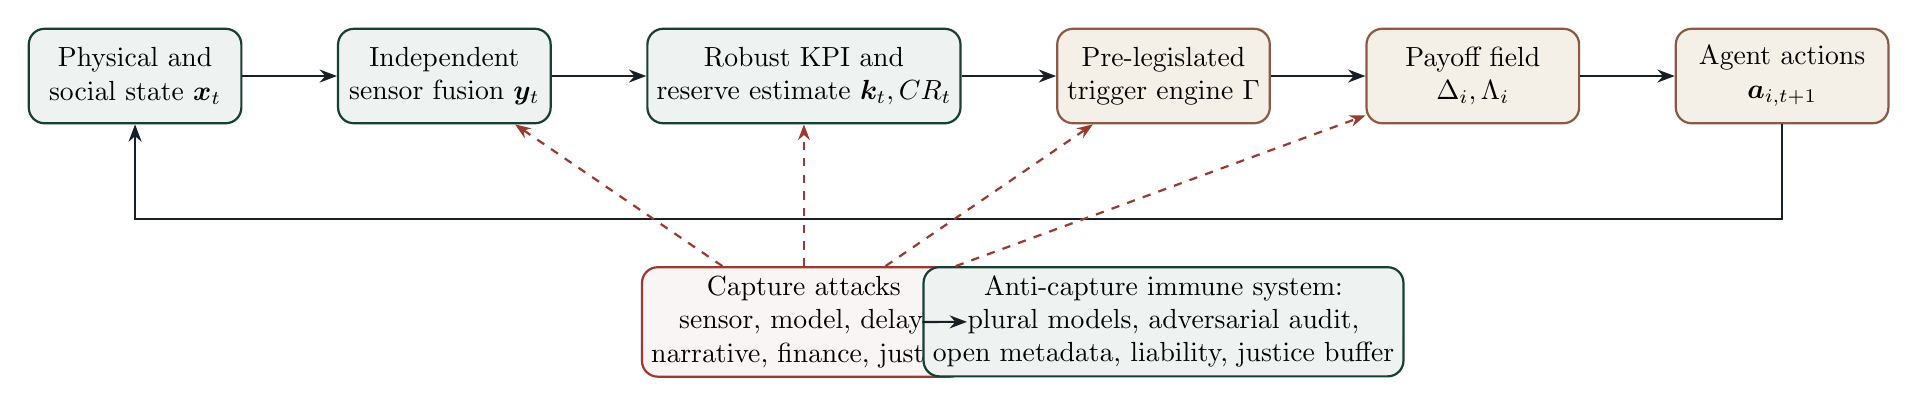
\begin{tikzpicture}[
  node distance=10mm and 12mm,
  box/.style={draw=Forest,rounded corners=2mm,thick,minimum height=12mm,minimum width=27mm,align=center,fill=Mist},
  act/.style={draw=Earth,rounded corners=2mm,thick,minimum height=12mm,minimum width=27mm,align=center,fill=Sand},
  risk/.style={draw=Rust,rounded corners=2mm,thick,minimum height=10mm,minimum width=25mm,align=center,fill=Rust!5},
  arrow/.style={-{Stealth[length=2.2mm]},thick,color=Ink},
  attack/.style={-{Stealth[length=2mm]},dashed,thick,color=Rust}
]
\node[box] (world) {Physical and\\social state $\state_t$};
\node[box,right=of world] (sense) {Independent\\sensor fusion $\bm y_t$};
\node[box,right=of sense] (kpi) {Robust KPI and\\reserve estimate $\kpi_t,CR_t$};
\node[act,right=of kpi] (trigger) {Pre-legislated\\trigger engine $\Gamma$};
\node[act,right=of trigger] (payoff) {Payoff field\\$\Delta_i,\Lambda_i$};
\node[act,right=of payoff] (agents) {Agent actions\\$\action_{i,t+1}$};

\draw[arrow] (world) -- (sense);
\draw[arrow] (sense) -- (kpi);
\draw[arrow] (kpi) -- (trigger);
\draw[arrow] (trigger) -- (payoff);
\draw[arrow] (payoff) -- (agents);
\draw[arrow] (agents.south) |- ++(0,-12mm) -| (world.south);

\node[risk,below=18mm of kpi] (capture) {Capture attacks\\sensor, model, delay,\\narrative, finance, justice};
\node[box,below=18mm of trigger] (immune) {Anti-capture immune system:\\plural models, adversarial audit,\\open metadata, liability, justice buffer};
\draw[attack] (capture) -- (sense);
\draw[attack] (capture) -- (kpi);
\draw[attack] (capture) -- (trigger);
\draw[attack] (capture) -- (payoff);
\draw[arrow] (immune) -- (capture);
\end{tikzpicture}%
}
\caption{Closed-loop architecture. The red dashed paths represent strategic attacks; the lower control path represents anti-capture defenses.}
\label{fig:architecture}
\end{figure}

% -----------------------------------------------------------------------------
\section{Observation Architecture and Ecological Sensing}
% -----------------------------------------------------------------------------

\subsection{A dashboard of non-fungible signals}

A practical KPI vector should contain physically and institutionally distinct signals rather than one composite score:
\begin{equation}
\kpi_t=
\left(
K_t^{E},K_t^{\mathrm{tail}},K_t^{\mathrm{infra}},K_t^{\mathrm{prod/finance}},
K_t^{\mathrm{bio}},K_t^{J},K_t^{\mathrm{capture}},K_t^{\tau}
\right).
\label{eq:dashboard}
\end{equation}
Representative components are real emissions and budget consumption; threshold exceedance frequency; infrastructure failure duration; fossil-production and financial-backflow gaps; ecosystem integrity; justice burden; detected capture; and response delay. The dashboard is not aggregated when aggregation would allow one improvement to compensate for an irreplaceable loss.

\subsection{Soundscape as one ensemble sensor}

Soundscape ecology distinguishes biophony, geophony, and anthrophony and provides a scalable method for observing ecological change \citep{pijanowski2011}. The Acoustic Complexity Index (ACI) measures temporal changes in intensity within frequency bins \citep{pieretti2011}. A schematic form is
\begin{equation}
\mathsf{ACI}=\sum_f
\frac{\sum_t |I_{f,t+1}-I_{f,t}|}
{\sum_t I_{f,t}+\epsilon}.
\label{eq:aci}
\end{equation}
The Normalized Difference Soundscape Index (NDSI) contrasts selected biophony and anthrophony bands:
\begin{equation}
\mathsf{NDSI}=\frac{B-A}{B+A+\epsilon}.
\label{eq:ndsi}
\end{equation}
Automated soundscape analysis has been used to track faunal recovery across tropical forest restoration gradients \citep{muller2023}. However, meta-analysis shows that acoustic indices are context-dependent proxies rather than universal measures of biodiversity \citep{alcocer2022}. Therefore
\begin{equation}
\widehat B_t=
\mathcal F_{\mathrm{eco}}
\left(
\text{soundscape},\text{eDNA},\text{remote sensing},
\text{field survey},\text{camera traps},\text{local knowledge}
\right),
\label{eq:ecosensorfusion}
\end{equation}
with uncertainty $\sigma_{B,t}$ and site-specific validation. The trigger should use posterior degradation probability, not raw loudness:
\begin{equation}
\Pp(B_t<B_{\mathrm{baseline}}-\delta\mid\bm y_{0:t})>p_{\mathrm{crit}}
\Longrightarrow \text{review or response}.
\label{eq:ecotrigger}
\end{equation}
Randomized sensor placement, hidden audit sensors, continuous sampling, playback anomaly detection, and protected access for sensitive species locations are part of the measurement design.

% -----------------------------------------------------------------------------
\section{Red-Team: How the New OS Will Be Gamed}
% -----------------------------------------------------------------------------

A governance model that assumes compliance after adoption is incomplete. Regulated actors adapt. Let the attack policy be
\begin{equation}
\policy_i^{\mathrm{hack}}\in\argmax_{m_i}
\left[
B_i^{\mathrm{rent}}+B_i^{\mathrm{delay}}+B_i^{\mathrm{legitimacy}}
+B_i^{\mathrm{access}}
-C_i^{\mathrm{penalty}}-C_i^{\mathrm{audit}}-C_i^{\mathrm{legal}}
\right].
\label{eq:hackutility}
\end{equation}
The target is often not physical improvement but maximal legal score at minimal transformation cost.

\begin{longtable}{@{}L{0.17\textwidth}L{0.34\textwidth}L{0.41\textwidth}@{}}
\caption{Representative attack--defense pairs.}\label{tab:redteam}\\
\toprule
\textbf{Attack surface} & \textbf{Realistic adaptation} & \textbf{Defense} \\
\midrule
\endfirsthead
\toprule
\textbf{Attack surface} & \textbf{Realistic adaptation} & \textbf{Defense} \\
\midrule
\endhead
Boundary laundering & Outsource or sell high-emission assets; reduce territorial or Scope 1 emissions while value-chain or consumption emissions rise. & Combine organizational, product, facility, consumption, and ownership accounting; retain transition responsibility after divestment for a defined period. \\
\addlinespace
Offset substitution & Purchase low-cost credits and present finance as direct abatement. & Separate reduction, removal, and contribution claims; restrict credits to verified residual emissions; impose additionality, durability, and double-counting liability. \\
\addlinespace
KPI cherry-picking & Improve carbon intensity while absolute emissions rise; emphasize renewable investment while fossil production expands. & Use mandatory KPI bundles, hard non-fungible floors, fixed core metrics plus rotating audit metrics, and absolute as well as intensity measures. \\
\addlinespace
Financial instrument gaming & Select easy sustainability targets, weak coupon penalties, or redemption before assessment. & Require material penalties, no early escape before target dates, independent baselines, absolute outcome metrics, and consequences beyond coupon adjustment. \\
\addlinespace
Trade circumvention & Re-route goods, alter product classification, split shipments, or supply low-emission lots only to regulated markets. & Facility-level product passports, beneficial-ownership tracking, anti-circumvention rules, and conservative default factors when traceability is absent. \\
\addlinespace
Soundscape theatre & Place sensors in favorable patches, shift disturbance outside sampling windows, or play recorded biophony. & Stratified randomized placement, continuous and surprise sampling, cross-sensor fusion, playback anomaly detection, and ecological composition metrics. \\
\addlinespace
Adaptation substitution & Claim adaptation expenditure while mitigation declines or carbon lock-in grows. & Score adaptation net of induced emissions, lock-in, burden transfer, and maladaptation; do not allow adaptation to offset mitigation backsliding. \\
\addlinespace
Justice backlash engineering & Concentrate transition costs on low-income households or dependent regions, then mobilize resulting opposition. & Couple every price or supply trigger to dividends, affordability floors, worker protection, regional investment, participation, and loss-and-damage finance. \\
\addlinespace
Legal delay & Use review, litigation, transition periods, and exceptions to postpone enforcement while rents continue. & Automatic default rules, expiry, escrowed liabilities, time-limited appeals, and explicit delay costs. \\
\addlinespace
Narrative capture & Reframe ``transition'' as indefinite preparation; use future technology promises to justify present expansion. & Evidence-backed claim standards, boundary disclosure, delivered-outcome accounting, legal liability, and zero credit for undelivered removals. \\
\addlinespace
Data flooding & Publish voluminous, incomparable reports that increase audit cost and hide material information. & Machine-readable minimum schemas, open metadata, facility-level data, independent assurance, auditor rotation, and public replication. \\
\addlinespace
Emergency-power capture & Use safety triggers to centralize authority indefinitely or suppress contestation. & Predefined release rules, judicial review, sunset clauses, rights floors, transparent models, and compensation for erroneous triggers. \\
\bottomrule
\end{longtable}

The attack catalogue implies six general defenses:
\begin{equation}
\mathsf{AntiCapture}=
\mathsf{Triangulation}+\mathsf{Automation}+\mathsf{Liability}
+\mathsf{AntiDelay}+\mathsf{Justice}+\mathsf{AdversarialAudit}.
\label{eq:anticapture}
\end{equation}
The effective capture term may be represented as
\begin{equation}
\capture_t^{\mathrm{eff}}=
\frac{\capture_t^{\mathrm{attempted}}}
{1+\mathsf{AntiCapture}_t+R_t^J+\mathsf{LegalExposure}_t}.
\label{eq:effectivecapture}
\end{equation}
This expression is schematic; its empirical content would require domain-specific estimation.

% -----------------------------------------------------------------------------
\section{Empirical Anchors and Claim Boundaries}
% -----------------------------------------------------------------------------

\begin{table}[H]
\centering
\caption{Selected empirical anchors. They motivate variables and failure modes but do not validate the full model.}
\label{tab:anchors}
\begin{tabularx}{\textwidth}{@{}L{0.27\textwidth}YL{0.25\textwidth}@{}}
\toprule
\textbf{Observation} & \textbf{Evidence} & \textbf{Model relevance} \\
\midrule
Non-punitive Paris compliance architecture & Article 15 and the PAICC specify a facilitative, non-adversarial, non-punitive mechanism \citep{unfccc2015,unfcccpaicc}. & Illustrates weak direct penalty coupling; does not imply that transparency and facilitation have zero value. \\
\addlinespace
Persistent policy-temperature gap & UNEP 2025 estimated 2.3--2.5\,\textdegree C under full NDC implementation and 2.8\,\textdegree C under current policy \citep{unep2025}. & Motivates separating commitments from physical trajectory. \\
\addlinespace
Fossil-production inconsistency & Governments collectively planned more than twice the 2030 production consistent with a 1.5\,\textdegree C pathway \citep{productiongap2025}. & Motivates a supply-side state and production-gap trigger. \\
\addlinespace
Record atmospheric concentrations & WMO reported 423.9 ppm globally averaged CO$_2$ in 2024 \citep{wmo2025}. & Anchors the physical state variable; concentration is not a complete welfare metric. \\
\addlinespace
Multiple Earth-system boundaries & Recent boundary assessments integrate climate, biosphere, water, nutrients, and justice \citep{rockstrom2023,richardson2023}. & Supports coupled constraints rather than a single temperature KPI. \\
\addlinespace
Context-sensitive acoustic indicators & Soundscape monitoring can track ecological recovery, while acoustic indices have limited universal proxy validity \citep{muller2023,alcocer2022}. & Supports ensemble sensing and explicit uncertainty rather than a single acoustic score. \\
\bottomrule
\end{tabularx}
\end{table}

The paper advances an architecture, not the following stronger claims:
\begin{itemize}
  \item It does not prove that the Paris Agreement was intentionally designed to fail.
  \item It does not identify one exact global recovery boundary.
  \item It does not assume that every actor is selfish, identical, or perfectly rational.
  \item It does not imply that punishment alone is optimal, or that all cooperation should be centralized.
  \item It does not treat soundscape indices as a universal biodiversity truth machine.
  \item It does not show that an automatic controller can resolve distributive conflict without politics.
\end{itemize}

% -----------------------------------------------------------------------------
\section{A Falsifiable Research Program}
% -----------------------------------------------------------------------------

\subsection{Minimal simulation environment}

A first implementation should be an agent-based partially observable stochastic game, not a full integrated assessment model. Let actors vary in economic dependence, power, exposure, externalization capacity, horizon, trust, and capture ability. Compare at least four governance arms:
\begin{enumerate}
  \item \textbf{Weak-coupling baseline}: observation and voluntary reporting with low $\partial\inst/\partial\kpi$.
  \item \textbf{Nominal trigger}: deterministic institutional response without capture defense.
  \item \textbf{Robust reserve controller}: ambiguity-aware triggers using $CR_t$ and viability constraints.
  \item \textbf{Full RVCIM}: robust triggers plus justice buffers, model plurality, adversarial audit, and accountable override.
\end{enumerate}

Key experimental sweeps include physical uncertainty, observation noise, common-mode model error, capture budget, policy delay, capital turnover, trust decay, and unequal transition burden. Outcomes include
\begin{align}
R_{\mathrm{irr}}(H)&=\Pp(\tau_{\irrev}^{(t)}\le H), \\
CR_{\min}&=\min_{t\le H}CR_t^{\mathrm{sys}}, \\
\mathsf{PG}_{\mathrm{cum}}&=\sum_{t\le H}\mathsf{PG}_t, \\
\mathsf{CA}&=1-\frac{\|\capture^{\mathrm{eff}}\|}{\|\capture^{\mathrm{attempted}}\|+\epsilon}, \\
\mathsf{JS}&=R_t^J-\mathsf{BacklashRisk}_t.
\end{align}
False-positive and false-negative trigger rates must both be measured. For irreversible risks, a false negative may have much greater cost, but excessive false positives can destroy legitimacy and thus future control capacity.

\subsection{Hypotheses}

\begin{hypothesis}[Coupling]
Holding physical dynamics, actor preferences, and capture fixed, increasing the credible KPI-to-payoff coupling $\Lambda_i$ for decisive actors reduces defective action relative to a monitoring-only baseline.
\end{hypothesis}

\begin{hypothesis}[Capture decay]
A nominal trigger initially improves outcomes but its effect decays under repeated strategic adaptation when capture is unmodeled; adversarial audit and function separation reduce that decay.
\end{hypothesis}

\begin{hypothesis}[Reserve advantage]
Under delayed and uncertain tipping dynamics, reserve-based triggers reduce entry into $\irrev$ relative to damage-threshold triggers, at the cost of a higher false-positive rate.
\end{hypothesis}

\begin{hypothesis}[Justice durability]
Transition policies with automatic justice buffers produce lower backlash, higher coordination reserve, and greater long-run policy persistence than otherwise identical punitive policies.
\end{hypothesis}

\begin{hypothesis}[Sensor ensemble]
A multimodal ecological observation ensemble is more robust to manipulation and domain shift than a single KPI, but remains vulnerable to common-mode model error.
\end{hypothesis}

\begin{hypothesis}[Adaptive path value]
Policies with staged commitments, signposts, and reversible early actions retain more option value under deep uncertainty than fixed long-horizon plans with equivalent expected benefits.
\end{hypothesis}

\subsection{Stress tests}

At minimum, evaluate scenarios in which: the boundary is 30\% closer than the median model; no reliable early warning appears; all models share a common bias; KPI data are accurate but institutions fail to act; institutions act but backlash forces repeal; an industry coordinates manipulation; two physical thresholds cascade; and emergency powers are captured. A design that succeeds only when all actors report honestly and all models are well calibrated is not an anti-capture architecture.

% -----------------------------------------------------------------------------
\section{Executable Reference and Feasibility Contract}
% -----------------------------------------------------------------------------

The repository companion turns the minimal research program into a small, inspectable experiment. Its purpose is to establish that the paper's formal pieces can be composed into one deterministic software loop and subjected to failure tests. Execution is an audit surface, not an evidentiary shortcut.

\subsection{Feasibility ladder and admissible claims}

The distinction between implementation and validation is organized as a four-level ladder. Progress at one level does not silently confer the claims of the next.

\begin{table}[H]
\centering
\small
\caption{Feasibility ladder for the manuscript and companion implementation.}
\label{tab:feasibility}
\begin{tabularx}{\textwidth}{@{}L{0.08\textwidth}L{0.24\textwidth}Y Y@{}}
\toprule
\textbf{Level} & \textbf{Object} & \textbf{Admissible claim} & \textbf{Additional evidence required to advance} \\
\midrule
F0 & Executable structural toy & The declared mechanisms compose into a coherent, inspectable, replayable loop under recorded conditions. & Deterministic tests, explicit assumptions, traceable outputs, and hash-addressed receipts anchored by a trusted manifest. \\
\addlinespace
F1 & Stylized calibrated model & A narrow mechanism reproduces selected regularities under documented assumptions. & Parameter provenance, identification argument, alternative mechanisms, sensitivity analysis, and held-out tests. \\
\addlinespace
F2 & Sectoral or jurisdictional shadow model & The system may support bounded, non-actuating analysis in a declared domain. & Scoped legal authority, live-data validation, distribution-shift monitoring, independent review, and prospective evaluation. \\
\addlinespace
F3 & Reversible institutional pilot & A specific mechanism is operationally feasible under declared safeguards. & Rights floor, appeal, compensation, rollback and release rules, accountable ownership, and measured real-world outcomes. \\
\bottomrule
\end{tabularx}
\end{table}

This release is F0. A successful run, an ordered comparison table, or a lower toy irreversible-entry rate cannot be promoted into a climate forecast, a causal policy estimate, or evidence that an institutional design is legitimate.

\subsection{Paper-to-code correspondence}

Table~\ref{tab:papertocode} makes the correspondence explicit enough to audit, while also stating where the implementation compresses the formal object.

\begin{table}[H]
\centering
\small
\caption{Correspondence between formal objects and the reference implementation.}
\label{tab:papertocode}
\begin{tabularx}{\textwidth}{@{}L{0.19\textwidth}L{0.31\textwidth}Y@{}}
\toprule
\textbf{Paper object} & \textbf{Implementation surface} & \textbf{F0 interpretation} \\
\midrule
$\state_t,\bm{s}_t$ & \texttt{WorldState} & Normalized physical pressure, biosphere, institution, trust, justice, policy, support, and audit state. \\
$\action_{i,t},\Delta_i$ & \texttt{actor\_actions()} & Heterogeneous payoff-sensitive cooperation, defection, capture, restoration, and symbolic action. \\
$\bm y_t,\kpi_t$ & \texttt{observe\_pressure()} & Noisy observation with manipulation and audit correction. \\
$\Theta_t$ & \texttt{Environment.model\_boundaries} & A finite model ensemble with common-mode bias and structural allowance. \\
$CR_t,\rho_t$ & \texttt{estimate\_reserve()} & Conservative estimated exit time minus endogenous response time. \\
$\Gamma$ & \texttt{select\_mode()}, \texttt{schedule\_policy()}, \texttt{advance\_policy()} & Trigger choice, delayed activation, and release logic. \\
$\capture_t^{\mathrm{eff}}$ & \texttt{effective\_capture\_value()} & Attempted capture after audit, function separation, justice, and policy exposure. \\
$\mathsf{PG}_t$ & Trace and episode accumulators & Symbolic action minus scaled verified physical improvement. \\
\bottomrule
\end{tabularx}
\end{table}

The code compares the four arms specified in the research program: weak coupling, nominal trigger, robust reserve, and full \RVCIM. Within an episode, all arms receive the same actor profiles, realized boundary, model errors, disturbances, observation noise, social noise, and random choice draws. This paired construction reduces internal comparison noise; it does not establish external validity.

\subsection{Reference implementation contract}

The executable contract is intentionally narrow and fail-closed:
\begin{enumerate}
  \item \textbf{Runtime.} The simulator uses Python 3.10 or newer and only the standard library. The checked-in source is the readable source of truth; execution does not depend on hidden payload assembly.
  \item \textbf{Declared input.} A run resolves \path{simulation/configs/minimal.json}, selected arms, episode count, seed, and command-line overrides into \path{resolved_config.json}. Unknown configuration keys are rejected.
  \item \textbf{Paired randomness.} The episode seed determines one common environment for all selected arms. Arm ordering cannot change the sampled exogenous episode.
  \item \textbf{Observable outputs.} Every complete run writes \path{summary.csv}, \path{episodes.csv}, \path{trace.csv}, \path{comparison.md}, \path{resolved_config.json}, and \path{receipt.json}. The receipt records the claim boundary, command, environment, source identity, configuration identity, and output hashes.
  \item \textbf{Verification.} Receipt verification resolves recorded paths relative to the receipt, recomputes SHA-256 identities, and returns non-zero for a missing or modified file. Repository verification also checks the release manifest and committed reference receipt, then replays the declared reference command and byte-compares its deterministic outputs.
  \item \textbf{Failure visibility.} False-positive and false-negative trigger rates are reported together. Skipped executable tests, absent release artifacts, and hash mismatches are failures, not successful partial results. Manuscript buildability is qualified separately with an explicit TeX toolchain and must not be inferred from Python CI.
\end{enumerate}

The reference command is:

\begin{lstlisting}[style=paperpseudo,language=bash]
python3 -m simulation run \
  --config simulation/configs/minimal.json \
  --episodes 64 --seed 7 \
  --out artifacts/reference_run --overwrite

python3 -m simulation verify \
  --receipt artifacts/reference_run/receipt.json
\end{lstlisting}

\begin{boundarybox}
\textbf{What F0 does not establish.} The normalized parameters are selected to expose an inspectable mechanism gradient. They do not estimate climate sensitivity, tipping distributions, institutional response, actor preferences, or real intervention effects. The executable establishes correspondence, replayability under the recorded source, configuration, seed, and compatible runtime, and falsifiable interfaces---not empirical truth, policy rank, safety, legality, or democratic legitimacy.
\end{boundarybox}

% -----------------------------------------------------------------------------
\section{Limitations and Open Problems}
% -----------------------------------------------------------------------------

First, the cooperative/defective partition is partly normative. An action can reduce emissions while violating justice or biodiversity constraints. The paper therefore requires plural hard constraints rather than a single climate score, but disagreements over those constraints remain political.

Second, robust worst-case methods can become excessively conservative. Ambiguity sets may contain implausible models, and powerful actors may weaponize uncertainty to block beneficial transformation. The response is not to ignore uncertainty but to combine hard safety constraints with safe learning, staged trials, explicit information value, and periodic model-set revision.

Third, institutional actuators do not behave like physical actuators. Enforcement depends on legitimacy, legal authority, implementation capacity, and interpretation. Equations such as \cref{eq:institution,eq:barrierchance} are formal abstractions that must be instantiated separately in each jurisdiction.

Fourth, automatic triggers create constitutional risk. Rules justified by an unknown boundary can be used to normalize emergency powers. Release conditions, rights floors, transparent models, independent appeal, compensation, and legislative renewal are therefore part of the controller, not optional safeguards.

Fifth, the robust viability kernel may be computationally intractable in high-dimensional coupled systems. Approximations, surrogate models, scenario discovery, and decomposition will be necessary. Model plurality can reduce single-model dependence but does not eliminate correlated error.

Sixth, physical stabilization after payoff inversion may be slow. A governance reform can be successful in strategic terms while concentrations, ice loss, or ecological damage continue due to lag. Evaluation must distinguish policy coupling, action change, and delayed physical response.

Finally, this paper has not estimated its parameters or demonstrated empirical superiority. It defines the variables, conditional claims, attack surfaces, and tests needed to do so.

% -----------------------------------------------------------------------------
\section{Conclusion}
% -----------------------------------------------------------------------------

Nash's Cage names a system in which local rationality, physical externalization, short horizons, partial observation, and institutional capture jointly stabilize collective degradation. The architecture is dangerous not only because the physical state worsens, but because it can shrink the future set of feasible recoveries. The decisive threshold may therefore precede visible collapse: remaining safe time becomes shorter than institutional and biophysical braking time.

\RVCIM responds by changing the order of operations. It does not maximize short-term welfare and then price the damage. It first constrains irreversible risk and injustice, then optimizes within the remaining viable region. It does not assume that a better dashboard is governance. It measures the full chain from observation to actuator, payoff, behavior, and physical response. It does not assume reform survives contact with regulated actors. Capture is a strategic state variable, and anti-capture design is an institutional immune system.

The manuscript's core proposition is deliberately conservative:
\begin{corebox}
When the irreversible boundary is unknown, governance should preserve the ability to brake rather than infer safety from the absence of visible collapse.
\end{corebox}

Observation without actuation is ritual. Actuation without justice is unstable. Optimization without preserved controllability is recklessness. The research question is therefore not simply whether the world is currently inside a nominal target. It is whether, across plausible models and real institutional delays, a feasible path back to a safe and just region still exists -- and whether the rules of the game make taking that path rational before the reserve is gone.

% -----------------------------------------------------------------------------
\appendix
\section{Notation Summary}
% -----------------------------------------------------------------------------

\begin{longtable}{@{}L{0.20\textwidth}L{0.72\textwidth}@{}}
\toprule
\textbf{Symbol} & \textbf{Meaning} \\
\midrule
$\state_t$ & Full physical, agent, institutional, and narrative state. \\
$\bm{s}_t$ & Physical and ecological state. \\
$\action_{i,t}$ & Actor $i$'s emissions, fossil, decarbonization, symbolic, capture, restoration, and adaptation actions. \\
$\inst_t$ & Institutional actuators and capacities. \\
$\narr_t$ & Narrative, awareness, trust, and legitimacy state. \\
$\bm y_t$ & Raw multimodal observations. \\
$\kpi_t$ & Institutional KPI and reserve dashboard. \\
$\capture_t$ & Capture vector attacking metrics, institutions, delay, narrative, justice, and finance. \\
$\Theta_t$ & Ambiguity set of plausible system models. \\
$\safe$ & Present-time safe and just constraint set. \\
$\mathcal V_t^{\mathrm{rob}}$ & Robust viability set under feasible common policies. \\
$\irrev$ & Functionally irreversible state set. \\
$\tau_{\mathcal A}^{(t)}$ & First-passage delay from decision time $t$ into set $\mathcal A$. \\
$\rho_t(H)$ & Robust recoverability over horizon $H$. \\
$CR_t$ & Remaining lower-bound exit time minus upper-bound response time. \\
$\Delta_i$ & Cooperation payoff minus defection payoff. \\
$\Lambda_i$ & KPI-to-payoff coupling strength. \\
$\mathsf{PG}_t$ & Symbolic action minus scaled verified physical improvement. \\
$R_t^J$ & Justice and legitimacy reserve. \\
$\mathsf{OWD}(a)$ & One-Way Door index for action $a$. \\
\bottomrule
\end{longtable}

% -----------------------------------------------------------------------------
\section{Minimal Control Loop}
% -----------------------------------------------------------------------------

\begin{lstlisting}[style=paperpseudo]
At each decision time t:

1. Observe:
   y_t <- independent multi-sensor observations

2. Update uncertainty:
   Theta_t <- update plausible models + structural-error allowance

3. Estimate state and reserves:
   k_t, V_rob_t, rho_t, CR_t <- robust inference(y_0:t, Theta_t)

4. Red-team the observation:
   k_robust <- sensor fusion - manipulation allowance + audit correction

5. Select mode:
   if rho_t < rho_min:
       mode <- loss minimization
   else if lower_bound(CR_t) <= 0:
       mode <- emergency braking
   else if CR_t is low or boundary uncertainty is high:
       mode <- precaution
   else:
       mode <- adaptive normal

6. Select policy:
   maximize durable welfare + information value + option value
   subject to:
       irreversible-risk <= epsilon
       justice reserve >= J_min
       prohibited non-fungible loss == 0

7. Trigger actuators:
   price, cap, permit, finance, restoration, dividend, compensation

8. Audit adaptation:
   search for metric, boundary, delay, narrative, finance, and justice hacks

9. Publish:
   observations, models, uncertainty, trigger, burdens, beneficiaries,
   override and release conditions

10. Require review_interval < controllability_reserve; otherwise increase review cadence.
\end{lstlisting}

% -----------------------------------------------------------------------------
\section{Cage-Inversion Constitutional Invariants}
% -----------------------------------------------------------------------------

\begin{enumerate}
  \item \textbf{Unknown is not zero.} Missing evidence is not a safety certificate.
  \item \textbf{No silent loss of controllability.} Reserve deterioration must itself be a trigger.
  \item \textbf{No compensation across irreplaceable boundaries.} Non-fungible losses cannot be converted into generic credits.
  \item \textbf{One-way actions carry the proof burden.} Irreversibility raises the required confidence of safety.
  \item \textbf{Delay has a price.} Appeal and review cannot be costless defection strategies.
  \item \textbf{Justice is a floor.} Aggregate benefit cannot erase intolerable burden concentration.
  \item \textbf{No single epistemic controller.} Measurement, modeling, triggering, auditing, and appeal are separated.
  \item \textbf{Override is temporary and expensive.} Exceptions require public reasons, expiry, review, compensation, and traceability.
  \item \textbf{Every emergency trigger has a release rule.} Safety governance cannot become an unbounded permanent exception.
\end{enumerate}

% -----------------------------------------------------------------------------
\printbibliography[heading=bibintoc,title={References}]

\end{document}
